\chapter{Logistik mit Zeitfenster}
\label{Logistik mit Zeitfenster}

\section{Saving mit Zeitfenster in Python}

Dieses Beispiel stellt eine vereinfachte Welt dar, welche mit $5$ Knoten/Kunden und $1$ Depot ausgestattet ist. 
Das gesamte Netzwerk wurde nicht voll vernetzt, wie in Abbildung \ref{fig:exampleNetzwerk} ersichtlich ist. 
\begin{figure}
\centering
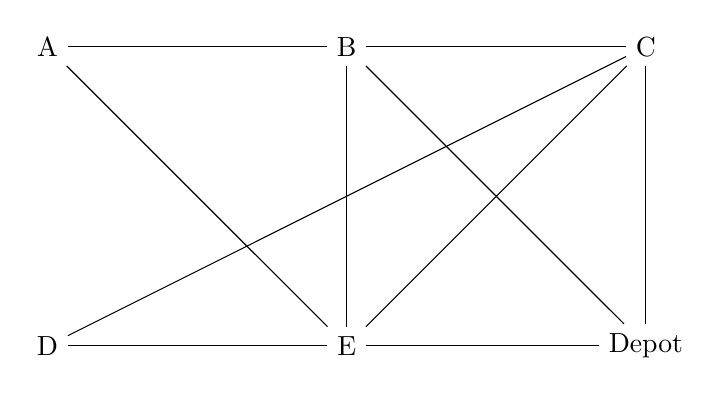
\begin{tikzpicture}[auto, node distance=3.8cm]
	
	\node (a) {A};
	
	\node (b) [right of=a] {B};
	
	\node (c) [right of=b] {C};
	
	\node (d) [below of=a] {D};
	
	\node (e) [right of=d] {E};
	
	\node (de) [right of=e] {Depot};
	
	\path 	(de) 	edge node {} (b)
					edge node {} (c)
			 		edge node {} (e)
			(a)		edge node {} (b)
					edge node {} (e)
			(b)		edge node {} (c)
					edge node {} (e)
			(c) 	edge node {} (d)
					edge node {} (e)
			(d)		edge node {} (e);
\end{tikzpicture}

	\caption{Beispiel Graph mit $5$ Knoten/Kunden und $1$ Depot}
	\label{fig:exampleNetzwerk}
\end{figure}
Aus diesem Grund muss der Knoten \textit{D} von \textit{A} oder \textit{B} aus über \textit{E} angefahren werden. 
Dies gilt auch für die Strecke vom Depot aus. 
Die Zeit- und Distanzmatrix sind in diesem Beispiel vollständig. 
So beinhalten sie auch die kombinierte Strecke von \textit{A $\rightarrow$ E $\rightarrow$ D} mit den aufsummierten Kosten. 
In Tabelle \ref{tab:edgeValues} sind alle benötigten Werte des Graphen \ref{fig:exampleNetzwerk} aufgeschlüsselt. 
Hierbei muss beachtet werden, dass die Zeit in Minuten und Sekunden angegeben ist. 
\begin{table}[htb]%[ht!]
\centering
\begin{tabular}{c|c|c|c}
%\hline 
Kante & km/h & km & Zeit (mm:ss) \\ 
\hline 
A $\leftrightarrow$ B & 80 & 10 & 07:30 \\ 
%\hline 
A $\leftrightarrow$ E & 100 & 14,14 & 08:29 \\ 
%\hline 
B $\leftrightarrow$ C & 90 & 10 & 06:40 \\ 
%\hline 
B $\leftrightarrow$ E & 110 & 10 & 05:27 \\ 
%\hline 
B $\leftrightarrow$ DE & 100 & 14,14 & 08:29 \\ 
%\hline 
C $\leftrightarrow$ D & 130 & 22,36 & 10:19 \\ 
%\hline 
C $\leftrightarrow$ E & 70 & 14,14 & 12:07 \\ 
%\hline 
C $\leftrightarrow$ DE & 100 & 10 & 06:00 \\ 
%\hline 
D $\leftrightarrow$ E & 90 & 10 & 06:40 \\ 
%\hline 
E $\leftrightarrow$ DE & 100 & 10 & 06:00 \\ 
%\hline 
\end{tabular} 
\caption{Aufschlüsselung der Distanzen, Durchschnittsgeschwindigkeiten und der benötigten Zeiten}
\label{tab:edgeValues}
\end{table}
Das Beispiel beinhaltet den gesamten Algorithmus \ref{list:algo}, welcher mit der Skriptsprache Python implementiert ist. 
Wie in einer Sektion zuvor schon beschrieben muss mit der Initialisierung begonnen werden. 
Hierzu müssen die Kostenmatrix sowie die trivialen Routen erstellt werden. 
Bei der Distanzmatrix ist zu beachten, dass diese in Kilometern beschrieben ist und intern auf Meter umgerechnet wird. 
Des Weiteren beinhaltet die Zeitmatrix die Zeiten bereits in Sekunden. 
In dieser Implementierung des Algorithmus werden alle Zeiten in Sekunden gerechnet inklusive der Wartezeiten. 

\noindent
Eine triviale Route beinhaltet nur einen Knoten, sodass die Strecke \textit{Depot $\rightarrow$ Knoten/Kunde $\rightarrow$ Depot} abgebildet wird. 
Weiters werden die möglichen Kombinationen erstellt und deren Ersparnis berechnet. 
Bei der Berechnung des Savings-Wertes muss die Nebenbedingung der Zeitfenster überprüft werden. 
Dieser erste Schritt erstreckt sich von Zeile $23$ bis Zeile $70$. 

\noindent
Im zweiten Schritt werden Routen kombiniert, bis keine Kombinationen mehr durchführbar sind. 
Dabei müssen nach der Kombination zweier Routen alle Einträge aus der Saving-Liste aktualisiert werden.
Zu diesen Aktualisierungsaufgaben zählen:
\begin{itemize}
	\item Entfernen aller Kombinationen, welche die zweite Route als Teil beinhalten;
	\item Ersetzen aller Routen in Kombinationen, welche die erste Route als Teil beinhalten;
\end{itemize}
Im Abschluss des zweiten Teils müssen die Ersparnisse mit überarbeiteten Routen neu berechnet und dabei die Zeitfenster geprüft werden. 
\lstinputlisting[language=Python,caption={Basis Implementierung des Saving-Algorithmus mit Zeitfenster},label=list:algo]{routing/routing.py}

\section{Ergebnis}

Gesamtheitlich kann festgestellt werden, dass eine grundsätzlich optimierte Route gefunden wurde. 
Trotzdem sieht es danach aus, als ob es noch bessere Routen geben müsste, wie im Ergebnis \ref{list:result} ersichtlich. 
Dabei muss wiederholt werden, dass es sich bei diesem Algorithmus um eine heuristische Lösung handelt. 
\lstinputlisting[caption={Ergebnis des Beispiels}, label=list:result, firstline=195]{routing/result.txt}

\noindent
Die Route \textit{Depot $\rightarrow$ E $\rightarrow$ D $\rightarrow$ A $\rightarrow$ B $\rightarrow$ C $\rightarrow$ Depot} spiegelt zusätzlich eine Eigenheit des Savings-Algorithmus wieder. 
Dazu muss die Historie genauer betrachtet werden. 
Wie im Listing \ref{list:firstMerge} zu erkennen ist, werden in der ersten Vereinigung die Routen mit den Knoten \textit{A} und \textit{B} kombiniert. 
Der Grund liegt in der Ersparnis, da Knoten, die weiter vom Depot entfernt sind und nahe beieinander liegen, einen hohen Wert erlangen. 
\lstinputlisting[caption={Erste Kombination von zwei Teilrouten}, label=list:firstMerge, firstline=69, lastline=78]{routing/result.txt}
Im Vergleich dazu bekommt die Vereinigung \textit{C $\leftrightarrow$ D} nur auf einen sehr niedrigen Wert. 
Dies kommt mit der großen Entfernung zwischen den Punkten zustande und der geringeren Entfernung zum Depot. 

\noindent
In einem direkten Vergleich der generierten Tour und einer manuell zusammengestellten Tour lässt sich feststellen, dass es eine bessere Route gibt. 
In der Tabelle \ref{tab:genTour} befinden sich die Zeit- und Distanzkosten der generierten Tour. 
\begin{table}[htb]%[ht!]
\centering
\begin{tabular}{c|c|c|c|c|c|c|c}
%\hline 
 & E & D & A & B & C & DE & Summe\\ 
\hline 
Zeit & 360 & 400 & 400 + 509 & 450 & 400 & 360 & 2879 s \\
%\hline 
Distanz & 10 & 10 & 10 + 14,14 & 10 & 10 & 10 & 74,14 km \\
%\hline 
\end{tabular} 
\caption{Benötigte Zeit und Strecke der generierten Tour}
\label{tab:genTour}
\end{table}
Die Tabelle \ref{tab:manTour} beinhaltet die Zeit- und Distanzkosten der manuellen erstellten Tour.
\begin{table}[htb]%[ht!]
\centering
\begin{tabular}{c|c|c|c|c|c|c|c}
%\hline 
 & C & D & E & A & B & DE & Summe\\ 
\hline 
Zeit & 360 & 619 & 400 & 509 & 450 & 509 & 2847 s \\
%\hline 
Distanz & 10 & 22,36 & 10 & 14,14 & 10 & 14,14 & 60,64 km \\
%\hline 
\end{tabular} 
\caption{Benötigte Zeit und Strecke der manuellen Tour}
\label{tab:manTour}
\end{table}
Im Vergleich lässt sich erkennen, dass die Kante \textit{C $\leftrightarrow$ D} mehr Zeit und Distanz mit sich bringt. 
Dafür wird die Kante \textit{D $\leftrightarrow$ E} nicht mehrfach benötigt. 
Der zeitliche Unterschied liegt bei $32$ Sekunden ohne Berücksichtigung der Wartezeiten. 
In Bezug auf den realen Straßenverkehr, kann dieser Wert vernachlässigt werden. 
Die berechnete Kostenmatrix führt in diesem Fall dazu, dass die Strecke und die Zeit optimiert werden. 
Sollte aber die Distanz minimiert werden, so müsste eine Distanzmatrix als Kostenmatrix verwendet werden. 
Eine andere Möglichkeit wäre die Berechnung der Kosten abzuändern, sodass sich die Distanzen stärker widerspiegeln. 

\chapter{Zusammenfassung}
\label{Zusammenfassung}

Routing in der Logistik bietet die Möglichkeit effizienter Auslieferungen zu erledigen. 
Dabei existieren allgegenwärtig Navigationssysteme wie Google Maps. 
Diese Lösungen liefern meist nur die Möglichkeit einfache \textit{point-to-point} Optimierungen durchzuführen. 
Diese Konsumentenlösungen verwenden ohne Internetzugang nur Offline-Daten ohne aktuelle Verkehrslagen zu berücksichtigen. 
Im Falle von Belieferungen wird eine höhere Abstraktion benötigt.
So muss nicht nur die Strecke zwischen den Haltepunkten optimiert werden, sondern auch die Reihenfolge dieser. 
Dies führt somit von \textit{point-to-point} Optimierungen, wie der Dijkstra-Algorithmus, zu Knoten/Kunden Optimierungen, wie dem \textit{Tabu-Search}. 

\noindent
Im Rahmen der Arbeit wurden einige Problemstellungen der Logistik aufgezeigt. 
Es wurden auch mögliche Lösungsansätze für solche Probleme gezeigt und beschrieben. 
Der Savings-Algorithmus mit seinen Eigenheiten wurde zudem genauer beschrieben. 
Des Weiteren stellen Kostenfunktionen eine zentrale Komponente in Routing-Algorithmen dar. 
Durch diese wird definiert, wie und nach was optimiert wird. 

\noindent
Der Einsatz von Optimierungen in der Logistik benötigt spezielle Algorithmen. 
Die Komplexität solcher Routing-Probleme stellt eine besondere Herausforderung dar. 
So kann in begrenzter Zeit nicht einfach das Optimum gefunden werden.
Eine Ausnahme besteht, wenn die Anzahl an Stopps so gering ist, dass alle Kombinationen getestet werden können. 
Aus dieser zeitlichen Einschränkung heraus werden meistens heuristische und meta-heuristische Lösungen verwendet. 
Somit werden Routing-Probleme, wie das \textit{Traveling Salesman Problem}, die Menschheit noch weiter beschäftigen. 